% !TeX program = xelatex
\documentclass[12pt, a4paper]{article}
\usepackage{xltxtra}

% ! Language and fonts !
\usepackage{polyglossia}
% language
\setmainlanguage{russian}
\setotherlanguage{english}
% fonts
\setmainfont[Ligatures=TeX]{CMU Serif}
\setromanfont[Ligatures=TeX]{CMU Serif} 
\setsansfont[Ligatures=TeX]{CMU Serif} 
\setmonofont[Ligatures=TeX]{CMU Serif} 
% set fonts to cyrillic
\newfontfamily{\cyrillicfont}[Ligatures=TeX]{CMU Serif}
\newfontfamily{\cyrillicfontrm}[Ligatures=TeX]{CMU Serif}
\newfontfamily{\cyrillicfonttt}[Ligatures=TeX]{CMU Serif} 
\newfontfamily{\cyrillicfontsf}[Ligatures=TeX]{CMU Serif} 
% rename pictures and tables
\addto\captionsrussian{
  \renewcommand{\figurename}{Рис.}
  \renewcommand{\tablename}{Табл.}
}
% math
\usepackage{unicode-math}
\setmathfont{TeX Gyre Termes Math}

% ! Document format !
\usepackage{comment}
\begin{comment}]
\usepackage{geometry} % Задаём поля:
\geometry{left=3cm} % левое — 3 см;
\geometry{right= 1.5cm} % правое — 1,5 см;
\geometry{top=2cm} % верхнее — 2 см;
\geometry{bottom=2cm} % нижнее — 2 см;
\usepackage{setspace} \onehalfspacing % Задаём «полуторный» межстрочный интервал.
\usepackage{indentfirst} % Автоматически добавляем отступ в каждый новый абзац.
\usepackage[all]{nowidow} % Пакет для борьбы с «висячими» строками абзацев, лучшая альтернатива переопределению \clubpenalty и \widowpenalty.
\usepackage{enumitem} % Настраиваем работу со списками:
\def\labelitemi{—} % задаём длинное тире как стандартный маркер ненумерованного списка;
\setlist{nolistsep} % убираем дополнительные отступы между элементами списка;
\usepackage{fancyhdr} % Настраиваем колонтитулы:
\pagestyle{fancy} % задаём макет страницы, отличный от стандартного;
\fancyhf{} % сбрасываем содержимое колонтитулов;
\renewcommand{\headrulewidth}{0pt} \renewcommand{\footrulewidth}{0pt} % убираем декоративные линии из колонтитулов;
\fancyfoot[C]{\thepage} % настраиваем расположение номера страницы в нижнем колонтитуле: L — слева, R — справа, C — по центру.
\addto\captionsenglish{\renewcommand{\partname}{}} % меняем имя главы
\setcounter{part}{-\maxdimen} % убираем счет глав
\usepackage{titlesec} % настраиваем заголовки частей документа:
\titleformat*{\section}{\newpage\normalsize\bfseries\centering} % настраиваем заголовок раздела; начинаем каждый раздел с новой страницы; размер шрифта — такой же, как во всем документе, начертание — полужирное, выравнивание  — по центру.
\end{comment}

% ! useful package !
\setlength{\mathsurround}{2pt}
\usepackage{mathtext}
\usepackage{booktabs,tabulary,tabularx,longtable}
\newcolumntype{M}[1]{>{\centering\arraybackslash}m{#1}} % resize row
\newcolumntype{N}{@{}m{0pt}@{}} % zero row
\usepackage{array} % for extrarowheight
\usepackage{varwidth} % for the varwidth minipage environment
\usepackage{graphicx} 
\usepackage{listings} 
\usepackage{color} 
\usepackage{xunicode}
\usepackage{ulem}

\usepackage{sectsty}

\allsectionsfont{\centering}
\setcounter{secnumdepth}{0}

\usepackage{multicol}
\usepackage{lipsum}
\usepackage{mwe}
\usepackage{float}
\usepackage{rotating}

\usepackage[left=2cm,right=2cm,top=2cm,bottom=2.5cm]{geometry}

\author{Круглов Иван, Кузнецов Илья} 
\title{\textbf{Jira}} 
\date{\today} 

\begin{comment}
\addto\captionsrussian{
  \renewcommand{\contentsname}
    {Мы будем исследовать такие функции как}
}
\end{comment}

\begin{document}

    % page 1
    \begin{Huge}
        \maketitle
    \end{Huge}
    \null
    \vfill
    \begin{turn}{-45} 
        \Huge{Сверстано в \XeLaTeX}
    \end{turn}
    % page 2
    \newpage
    \tableofcontents
    
    % page 3
    \newpage
    \section{Краткий обзор}
    Jira - лидер на рынке. Большинство компаний используют именно ее и тому есть
    достаточное количество подтверждений, которое выходит за рамки обзора продукта.
    Некоторые также считают, что Jira является стандартом на данный момент.
    Рассмотрим совокупность факторов, которые могут быть критериями выбора именно Jira:
    \begin{itemize}
        \item Способность регистрировать связи между задачами «многие ко многим»
        \item Гибкость настроек "из коробки"
        \item Сохранение истории всех изменений по проекту
        \item Отчасти открытая архитектура и возможность доработки под собственные нужды
        \item Возможность сопряжения с внешними системами (GitHub, GitLab, SharePoint, etc)
        \item Возможность использования на своем сервере (для закрытых проектов)
    \end{itemize}
    Таким образом, это весьма сильный и гибкий инструмент, способный помочь каждой команде, 
    несмотря на его внешнюю сложность.
    \begin{figure}[H]
        \centering
        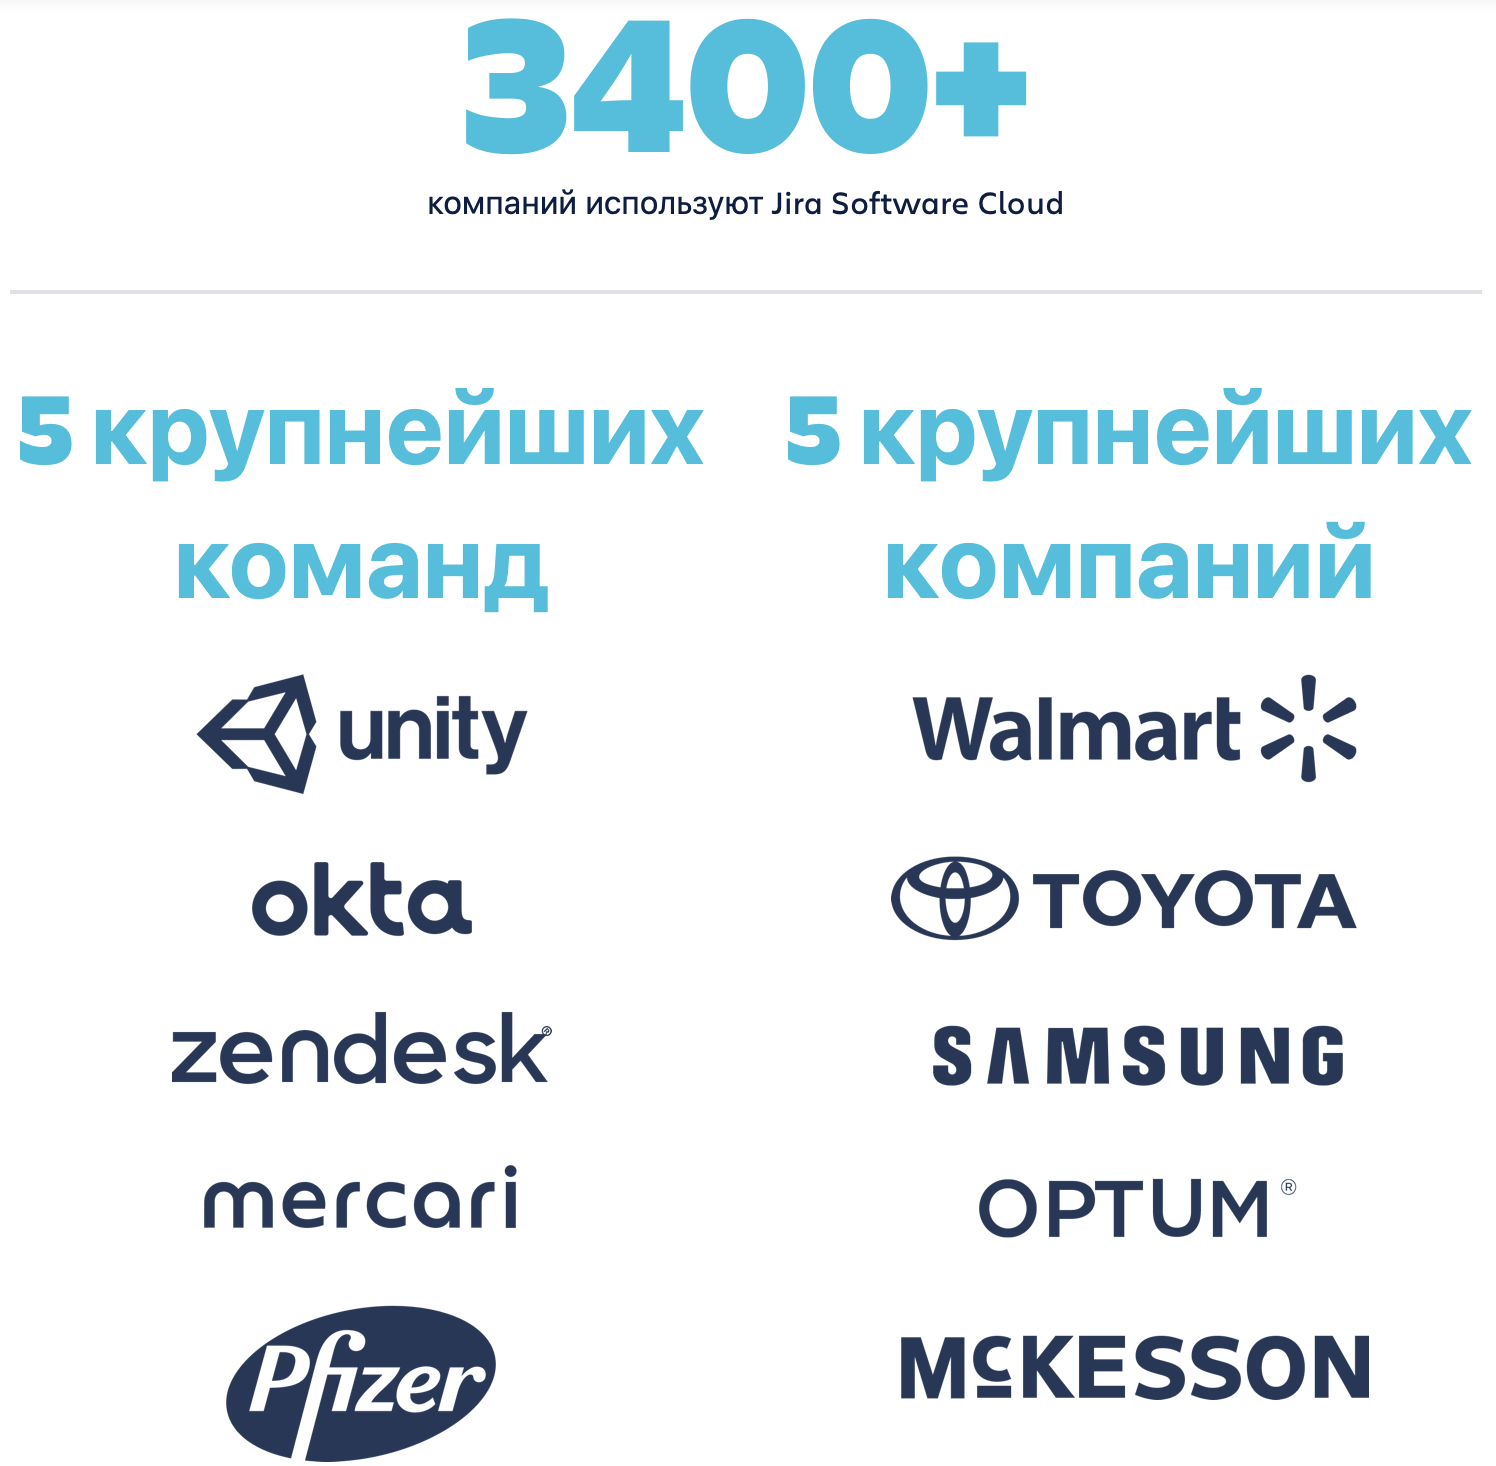
\includegraphics[width=0.75\linewidth]{src/1.png}
        \caption{Jira}
    \end{figure}


    % page 4
    \newpage
    \section{Создание проекта}
    Для создания проекта мы можем использовать 2 шаблона, каждый из которых является
    представителем Agile-методологии:
    
    \begin{multicols}{2}
        \subsection{Kanban}

        \begin{itemize}
            \item Не существует как таковых итераций, задачи можно подсовывать хоть каждый день
            \item Дает больше гибкости, если под гибкостью понимать частоту смены приоритетов.
            \item Здесь нет понятия «скорость работы команды», считается только среднее время на задачу.
            \item Целью является не законченный спринт, а законченная задача 
            \item Позволяет экстренно переключаться на другие задачи, которые не были запланированы
        \end{itemize}
        
    \columnbreak

        \subsection{Scrum}

        \begin{itemize}
            \item Основу составляют короткие итерации и спринты
            \item Перед началом спринта каждая команда формирует список задач
            \item После окончания спринта выполненные фичи заливаются на продакшн, 
            а невыполненные — переносятся в другой спринт
            \item Как правило, фичи, которые делаются во время спринта, не меняются: 
            что было на старте спринта — должно быть сделано любой ценой к окончанию спринта.
            \item Задачи принято оценивать в Story points или в часах
        \end{itemize}

    \end{multicols}

    \begin{figure}[H]
        \centering
        
\includegraphics[width=\linewidth]{src/scrumkanban.png}
        \caption{Создание проекта}
    \end{figure}

    Так же нам предлагается выбрать, кем будет управляться проект: командой или же компаний.
    Мы выберем Kanban и "управление командой"


    % page 5
    \newpage
    \section{Общий вид проекта}
    \begin{figure}[H]
        \centering
        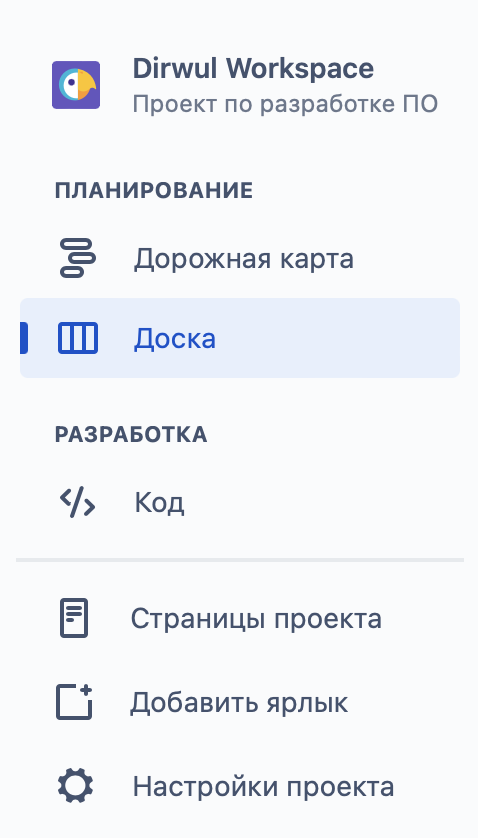
\includegraphics[width=0.3\linewidth]{src/preferences.png}
        \caption{Настройки проекта}
    \end{figure}
    В левом углу располагаются настройки проекта и вкладки:
    \begin{itemize}
        \item Roadmap - графический таймлайн для задач 
        \item Доска - непосредственно доски с задачами, как правило, именованые "к выполнению"/"в работе"/"готово"
        \item Код - вкладка с подключением системы контроля версий и возможностью просмотреть уже написанный код 
        \item Confluence — это пространство для командной работы, удобное для распределенных команд 
        Здесь накопленные командой знания объединены с возможностями для совместной работы
        \item Настройки проекта - это настройки внутреннего устройства всего нашего проекта, устройство задач и досок
    \end{itemize}

    
    % page 6
    \newpage
    \section{Основная функциональность}
    \subsection{Доска}
    На панели у нас представлено 3 карточки:
    \begin{itemize}
        \item К выполнению \textit{(запланированные задачи)}
        \item В работе \textit{(задачи в работе)}
        \item Готово \textit{(выполненные задачи)}
    \end{itemize}
    \begin{figure}[H]
        \centering
        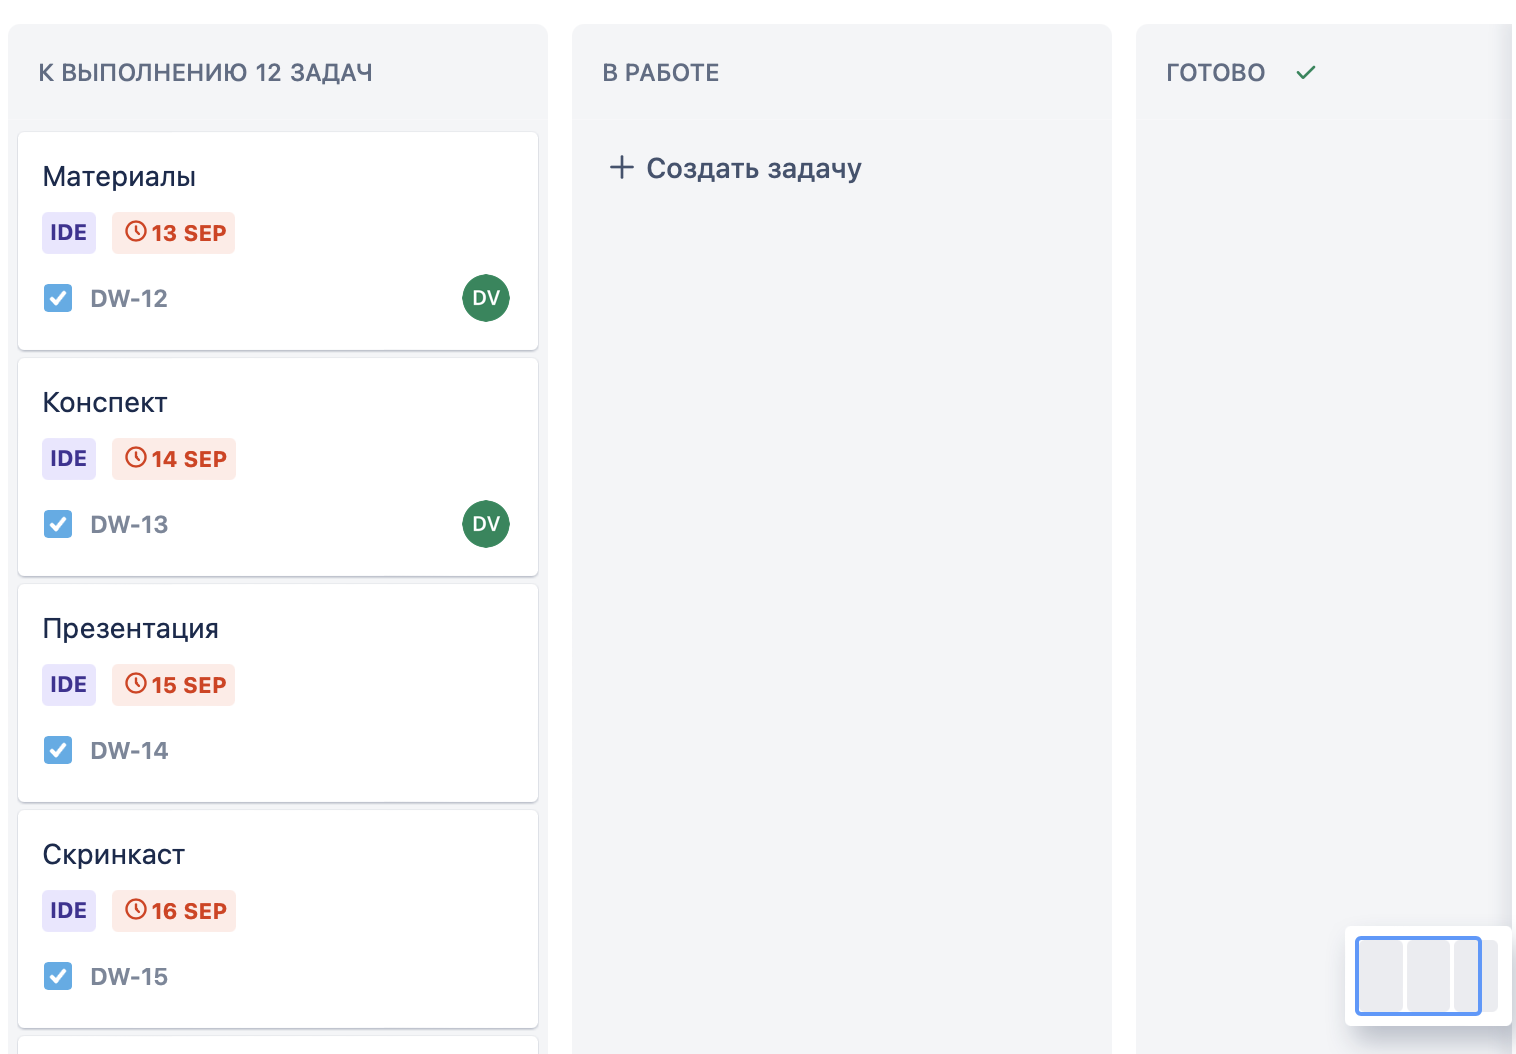
\includegraphics[width=0.75\linewidth]{src/desk.png}
        \caption{Карточки}
    \end{figure}
    Здесь мы можем создать задачу в любой из карточек, однако, как правило задачи создаются в карточке "к выполнению", 
    после чего перетаскиваются в следующую карточку.
    Таким образом легко проследить в какой момент времени задача имеет какой-либо из статусов.
    Большую задачу

    % page 7
    \newpage
    \subsection{Задача}
    Каждая задача может иметь время выполнения, быть помеченной, назначенной кому-то.
    Мы также можем создавать подзадачи к определенной задаче или же ссылаться на родительскую задачу.
    Функционал достаточно велик.
    \begin{multicols}{2}
        \begin{figure}[H]
            \centering{
\includegraphics[width=\linewidth]{src/task.png}}
            \caption{Задача}
        \end{figure}
        \columnbreak
        \begin{figure}[H]
            \centering{
\includegraphics[width=\linewidth]{src/taskpref.png}}
            \caption{Настройки задачи}
        \end{figure}
    \end{multicols}
    Нетрудно заметить, что в задаче все отображается довольно минималистично и понятно, что позволяет
    легко искать глазом нужную.
    Так же существует опция показать только те задачи, исполнитель которых назначен на определенного человека
    или нескольких \textit{(для этого достаточно нажать на иконки определенных людей, которые находятся
    чуть выше карточек, чьи задачи мы хотим просмотреть)}
    \begin{multicols}{2}[]
        \begin{figure}[H]
            \centering{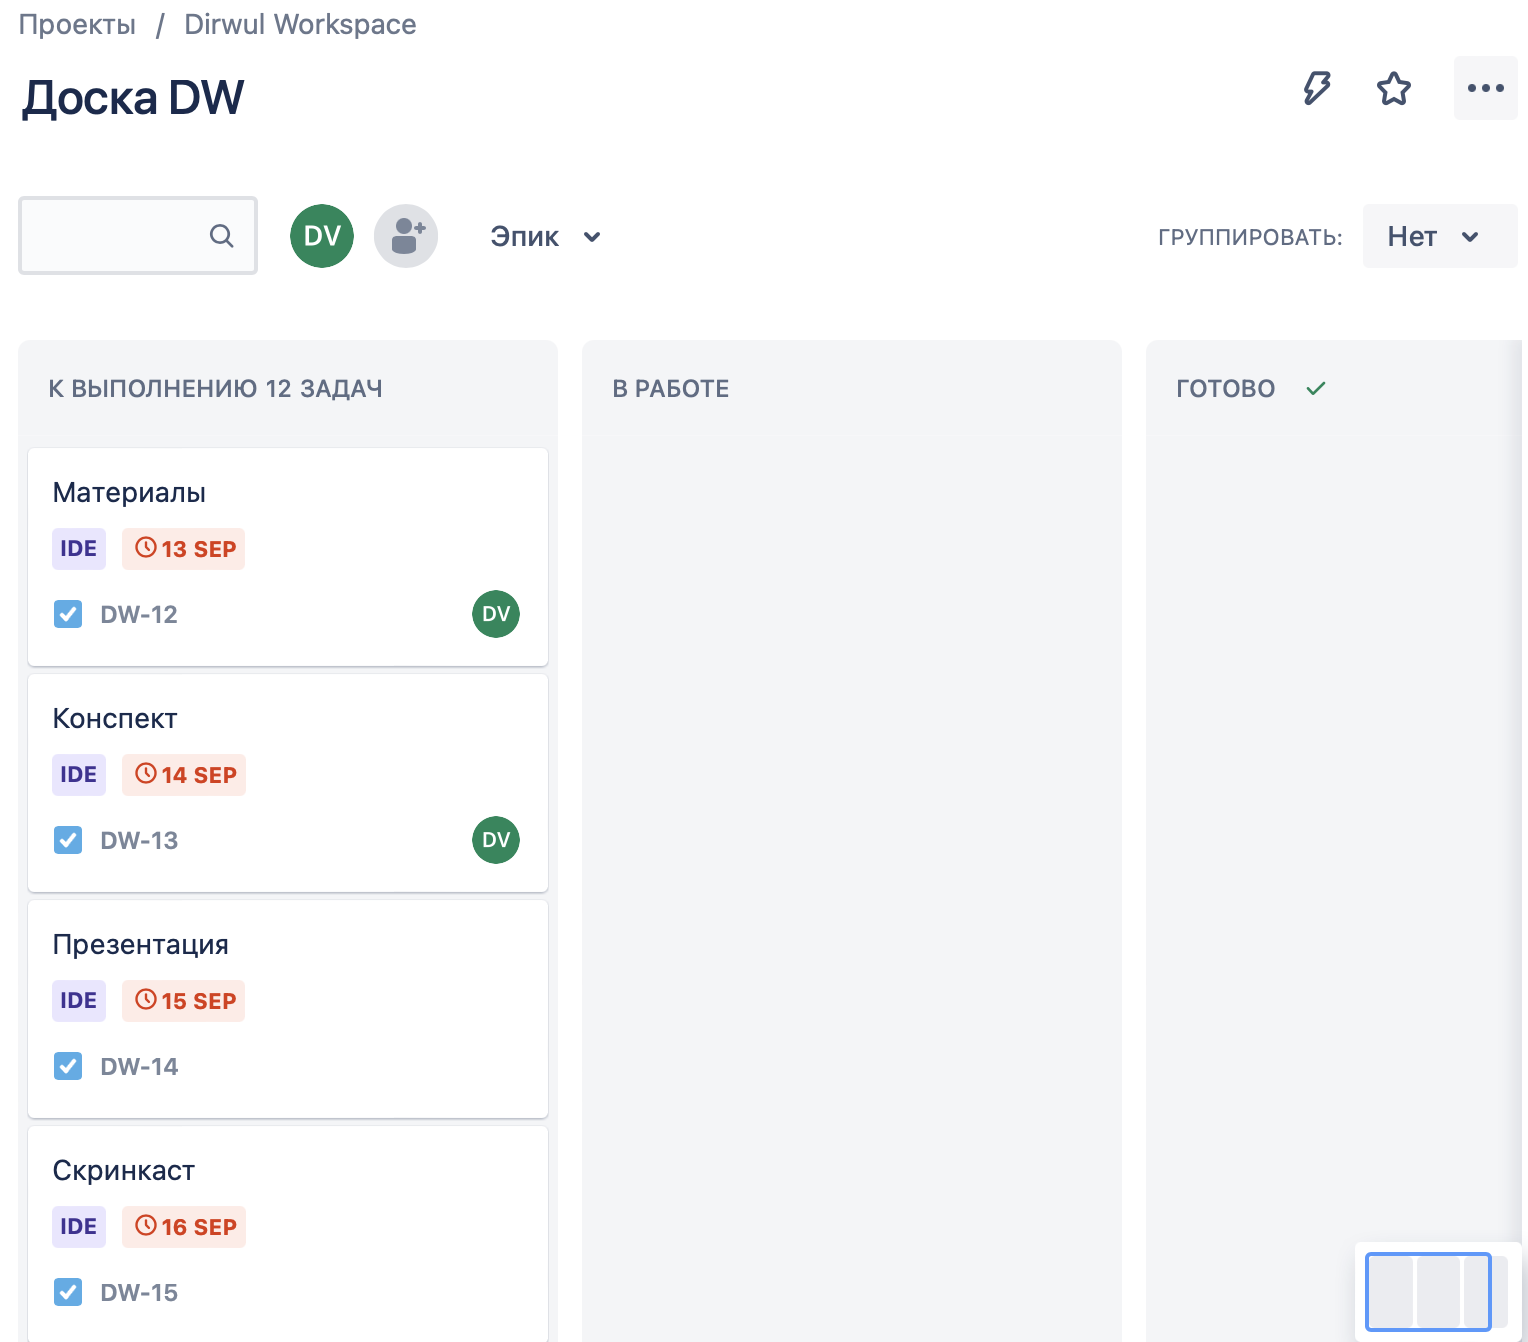
\includegraphics[width=\linewidth]{src/nosort.png}}
            \caption{Без сортировки по исполнителю}
        \end{figure}
        \columnbreak
        \begin{figure}[H]
            \centering{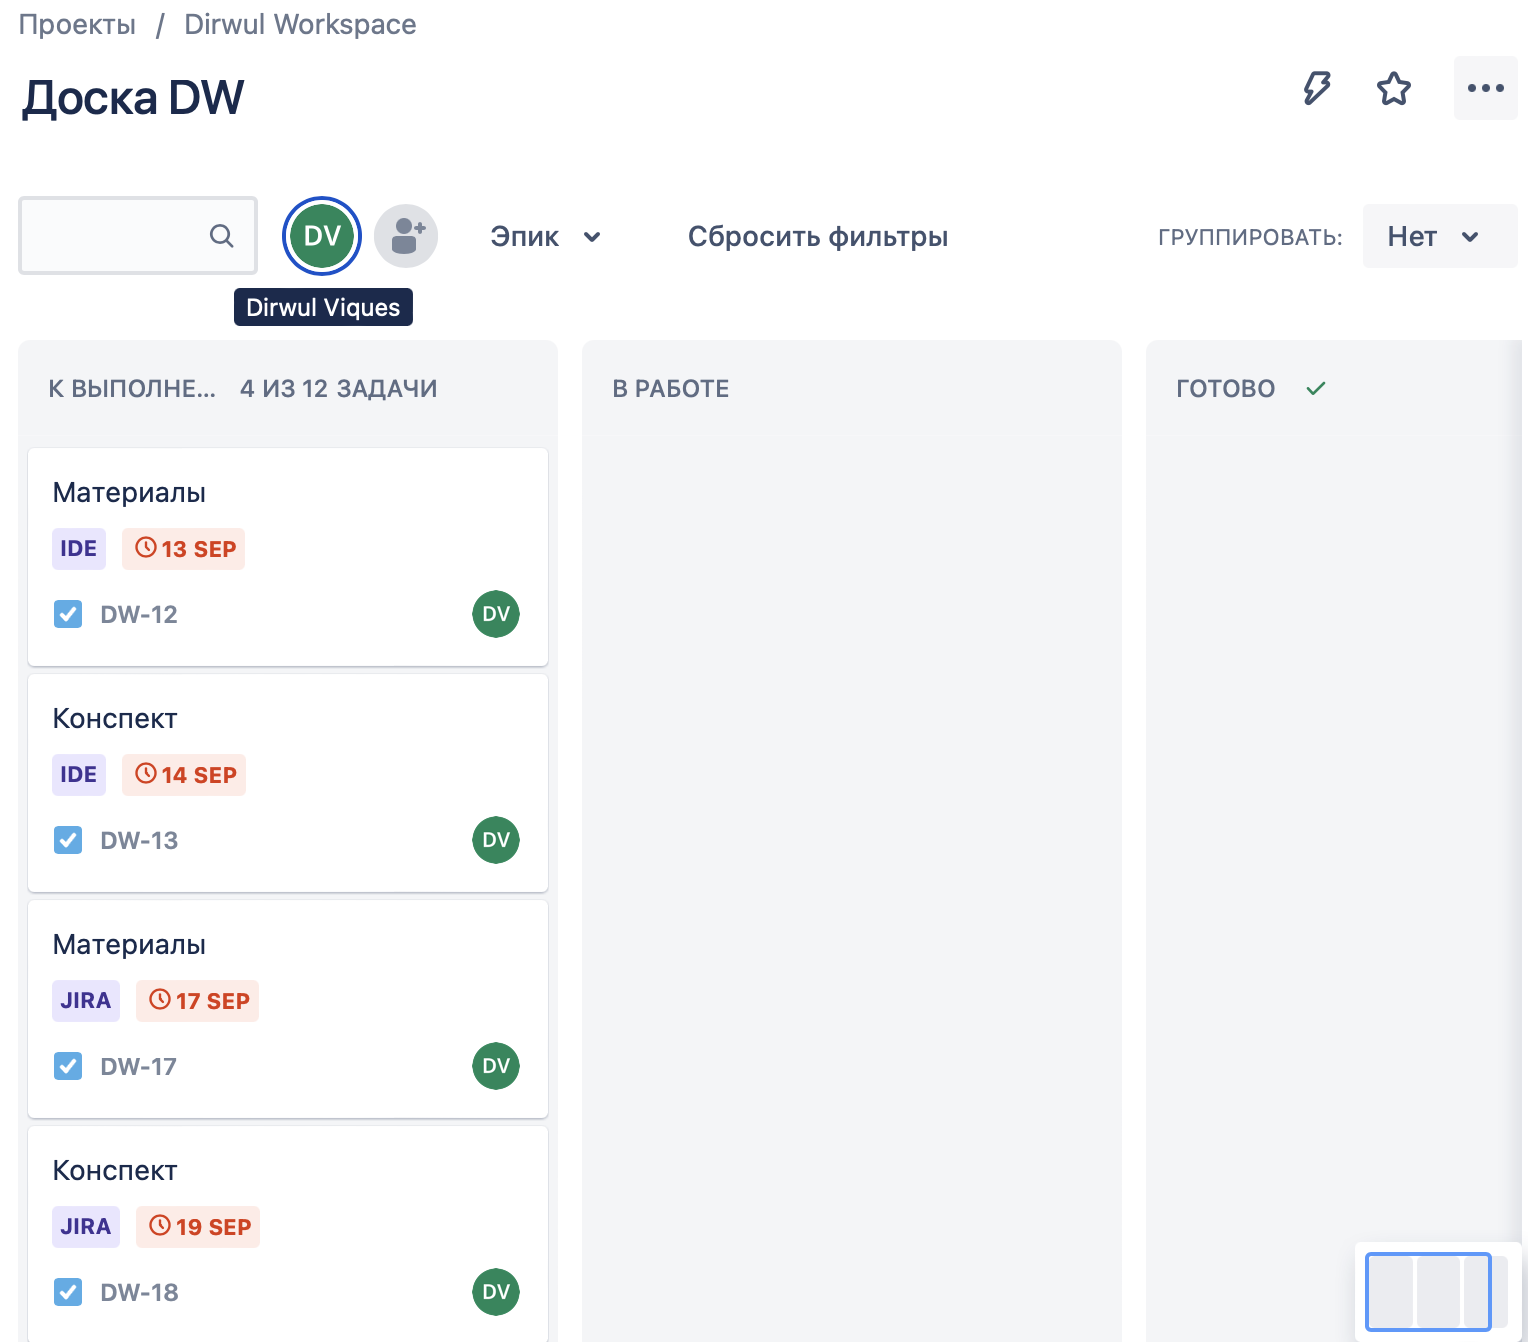
\includegraphics[width=\linewidth]{src/sort.png}}
            \caption{С сортировкой}
        \end{figure}
    \end{multicols}


    % page 8
    \newpage
    \subsection{Roadmap}
    В разделе дорожных карт мы можем делать все то же самое, что и в разделе "доска", разве что с другим интерфейсом,
    который позволяет распределить время на ту или иную задачу, но не смотреть на каждую задачу по отдельности
    \begin{multicols}{2}[]
        \begin{figure}[H]
            \centering{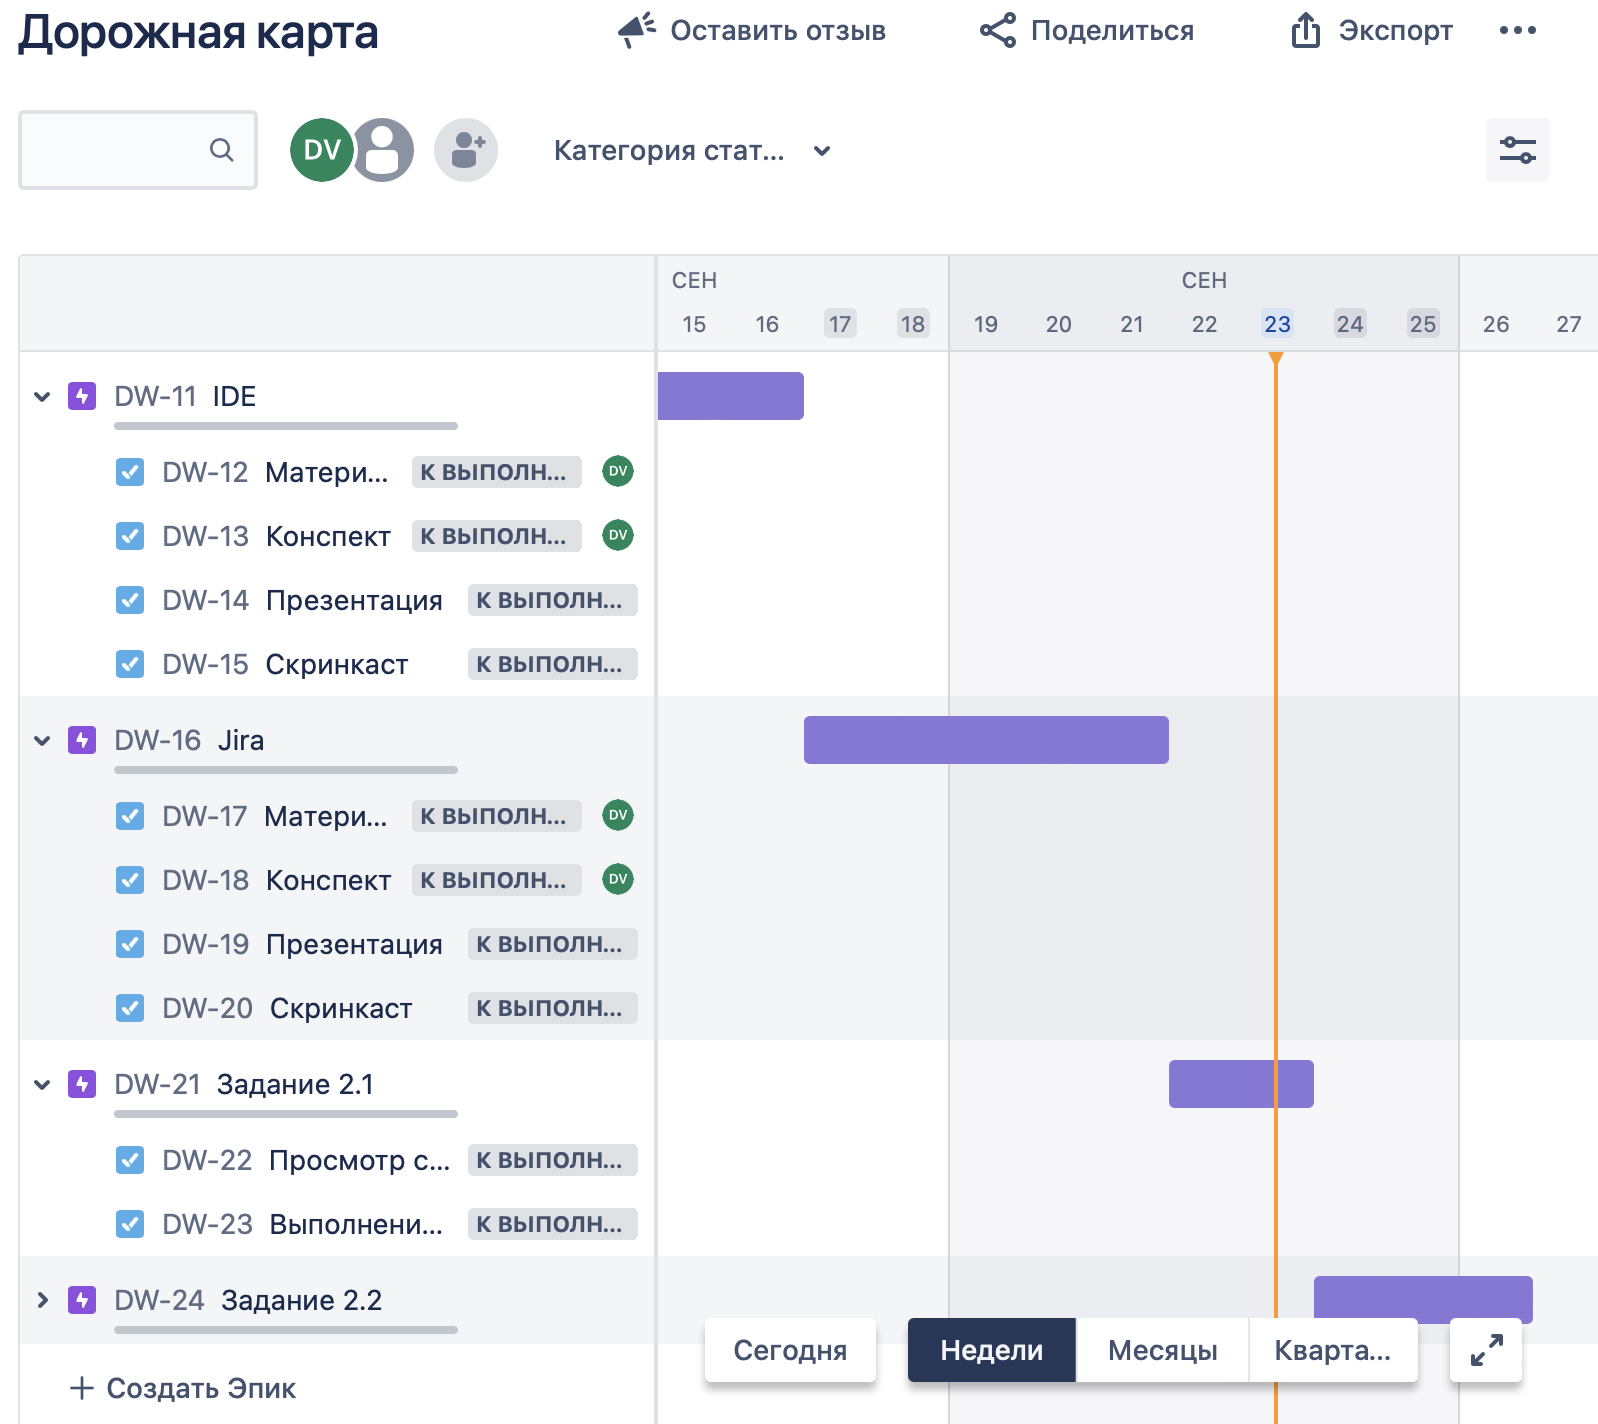
\includegraphics[width=\linewidth]{src/nosortroad.png}}
            \caption{Без сортировки по исполнителю}
        \end{figure}
        \columnbreak
        \begin{figure}[H]
            \centering{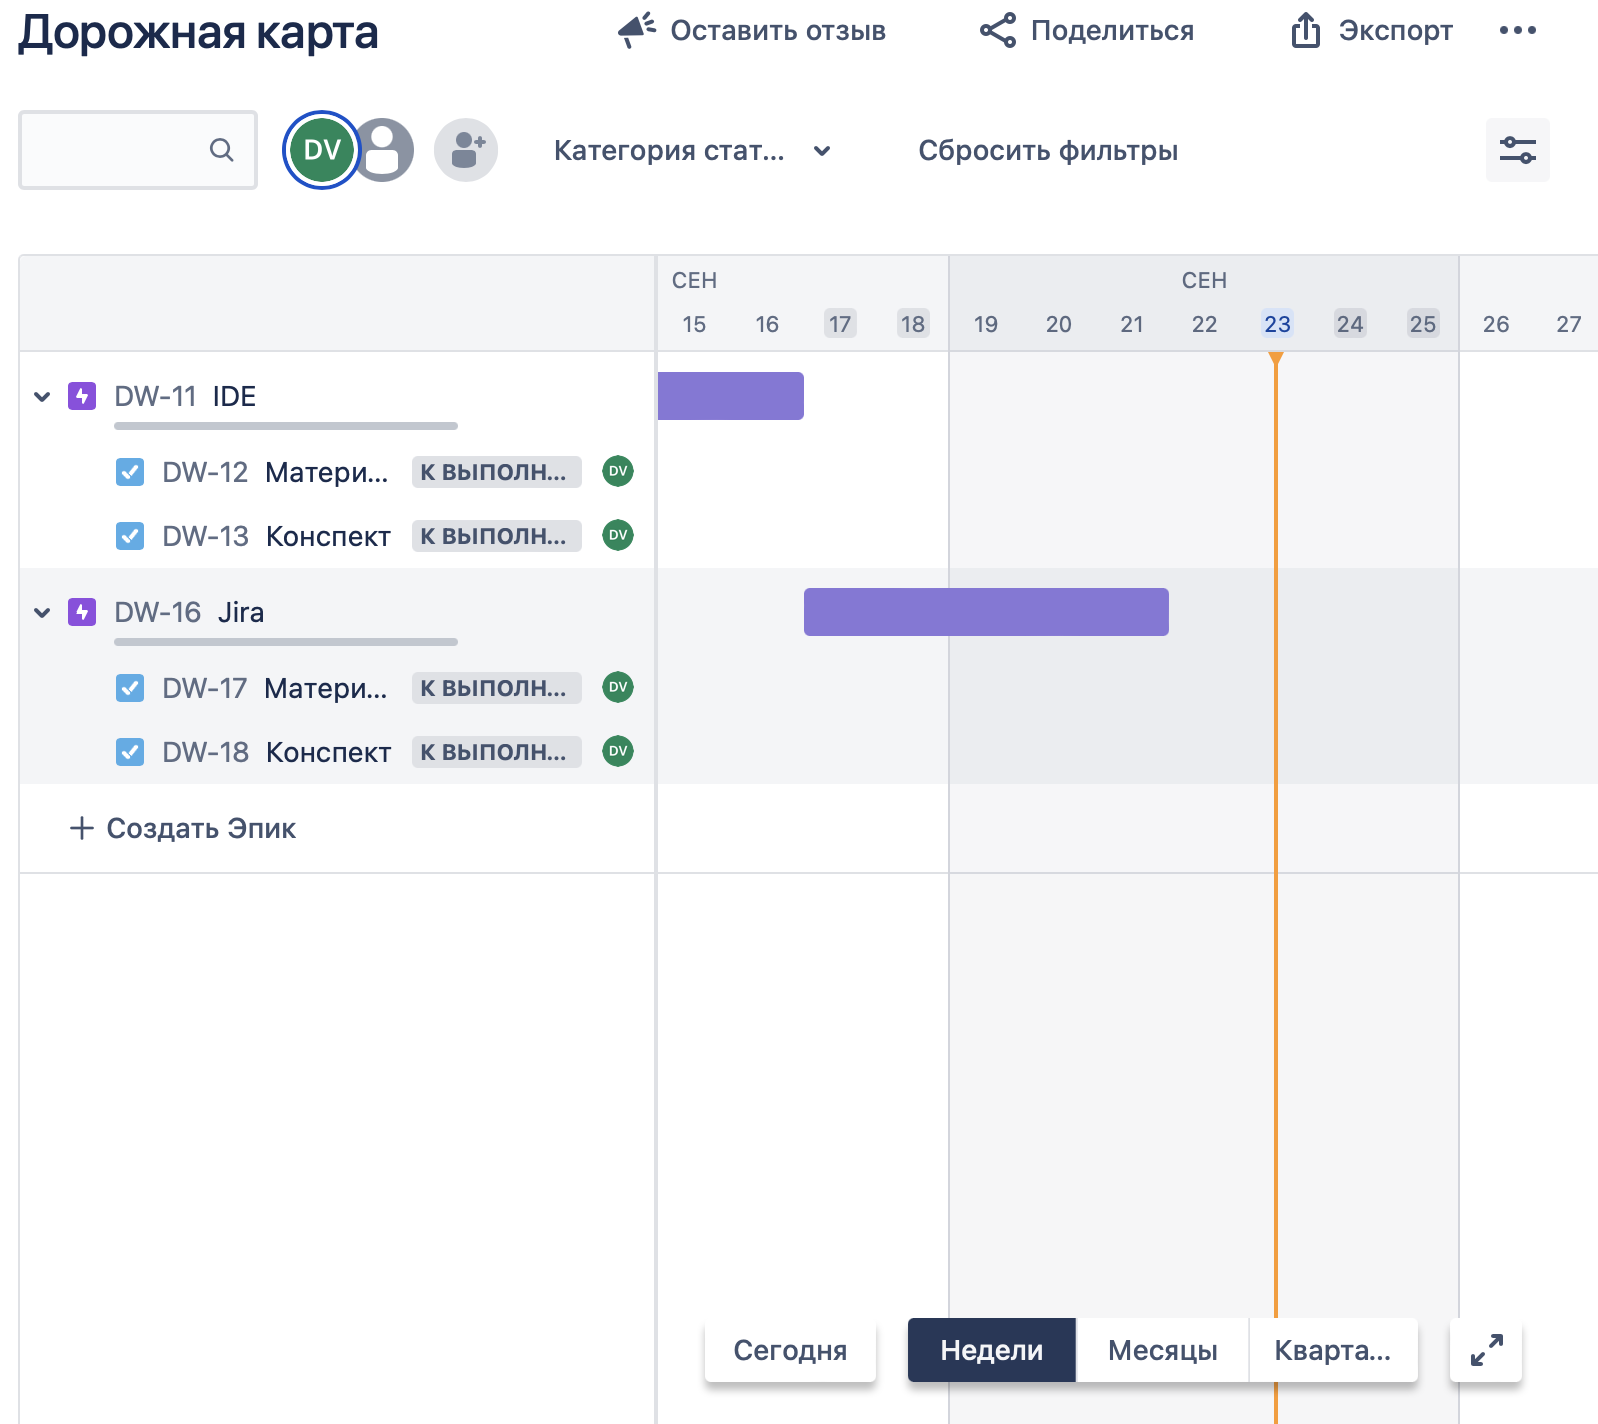
\includegraphics[width=\linewidth]{src/sortroad.png}}
            \caption{С сортировкой}
        \end{figure}
    \end{multicols}


    % page 9
    \subsection{Пресеты и полезные функции}
    Рассмотрим последний элемент, который нас может интересовать, если не углубляться в тонкости 
    инструментария Jira: верхнее табло, где находится полезная информация в более сжатом виды,
     пресеты и возможность подключать дополнительный инструментарий.
    
    \begin{multicols}{2}[]
        \begin{figure}[H]
            \centering{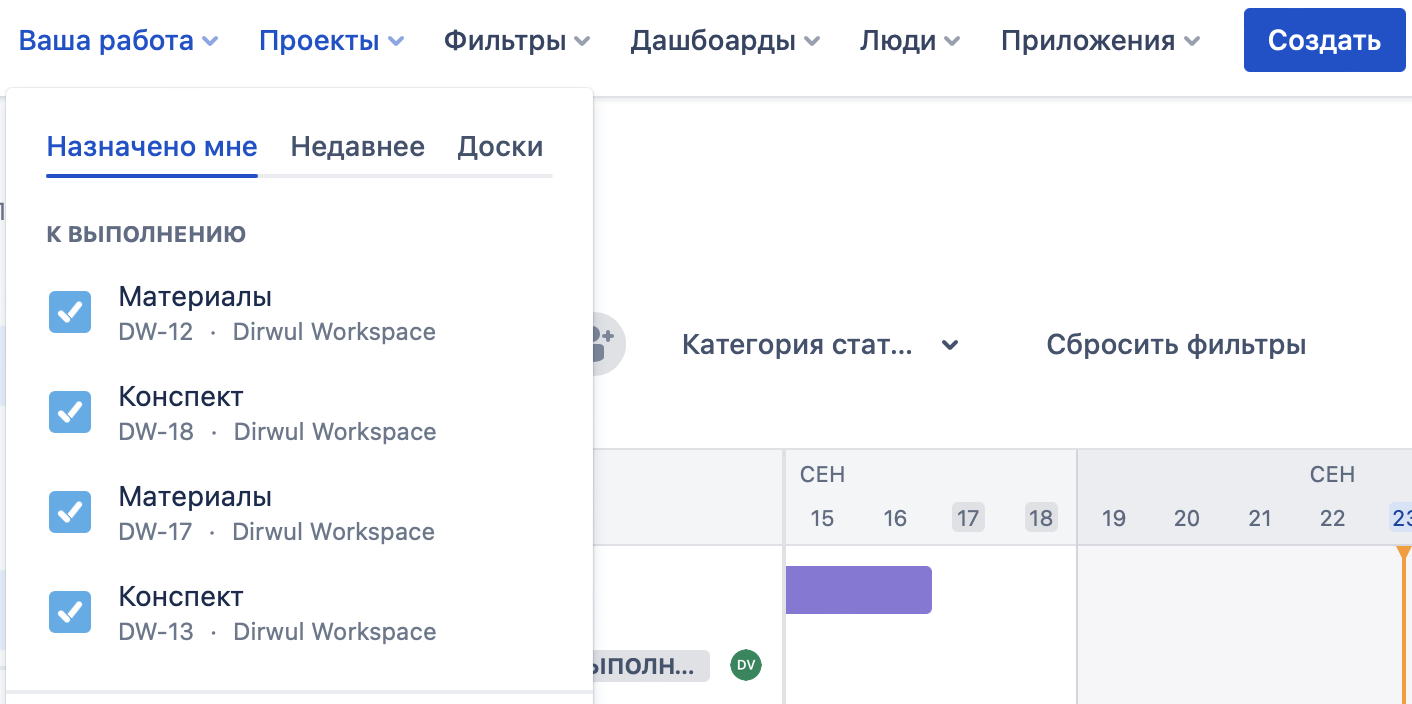
\includegraphics[width=\linewidth]{src/top1.png}}
            \caption{Работа}
        \end{figure}
        \columnbreak
        \begin{figure}[H]
            \centering{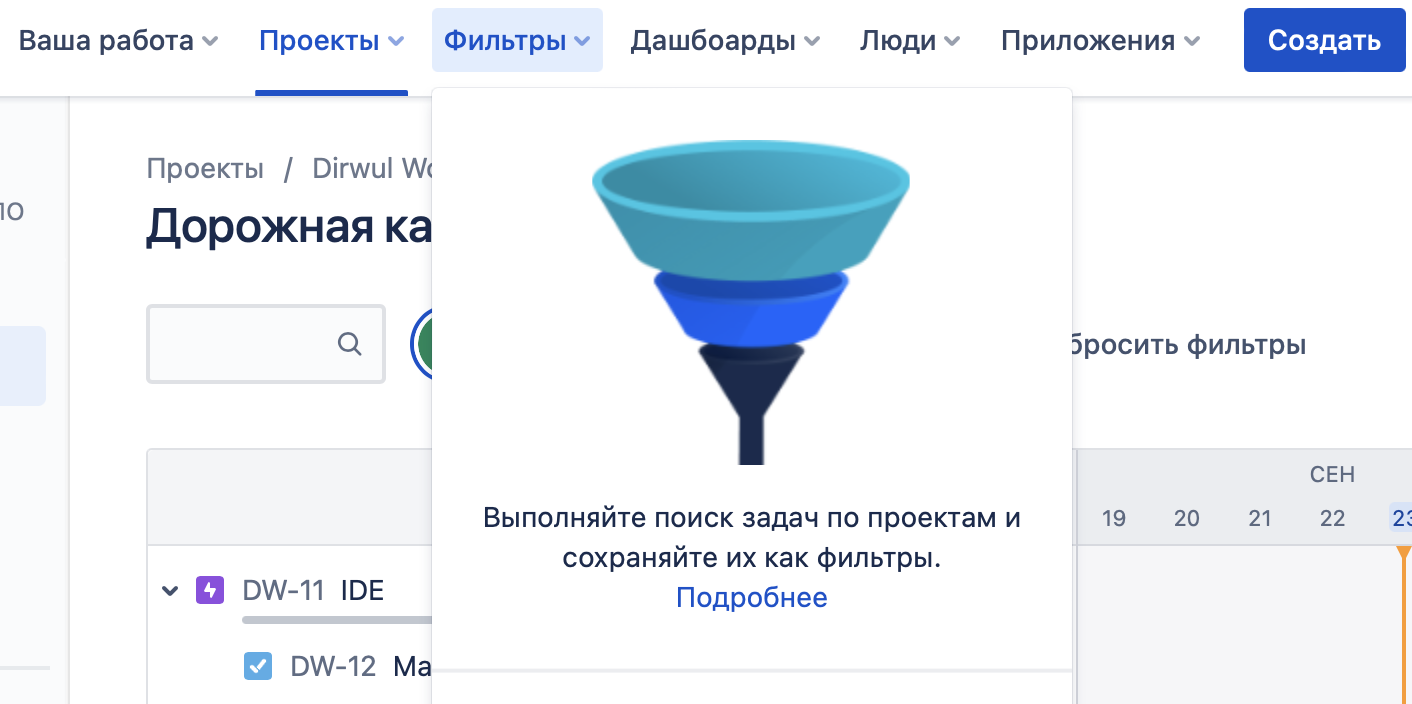
\includegraphics[width=\linewidth]{src/top2.png}}
            \caption{Фильтры}
        \end{figure}
    \end{multicols}
    \begin{multicols}{2}[]
        \begin{figure}[H]
            \centering{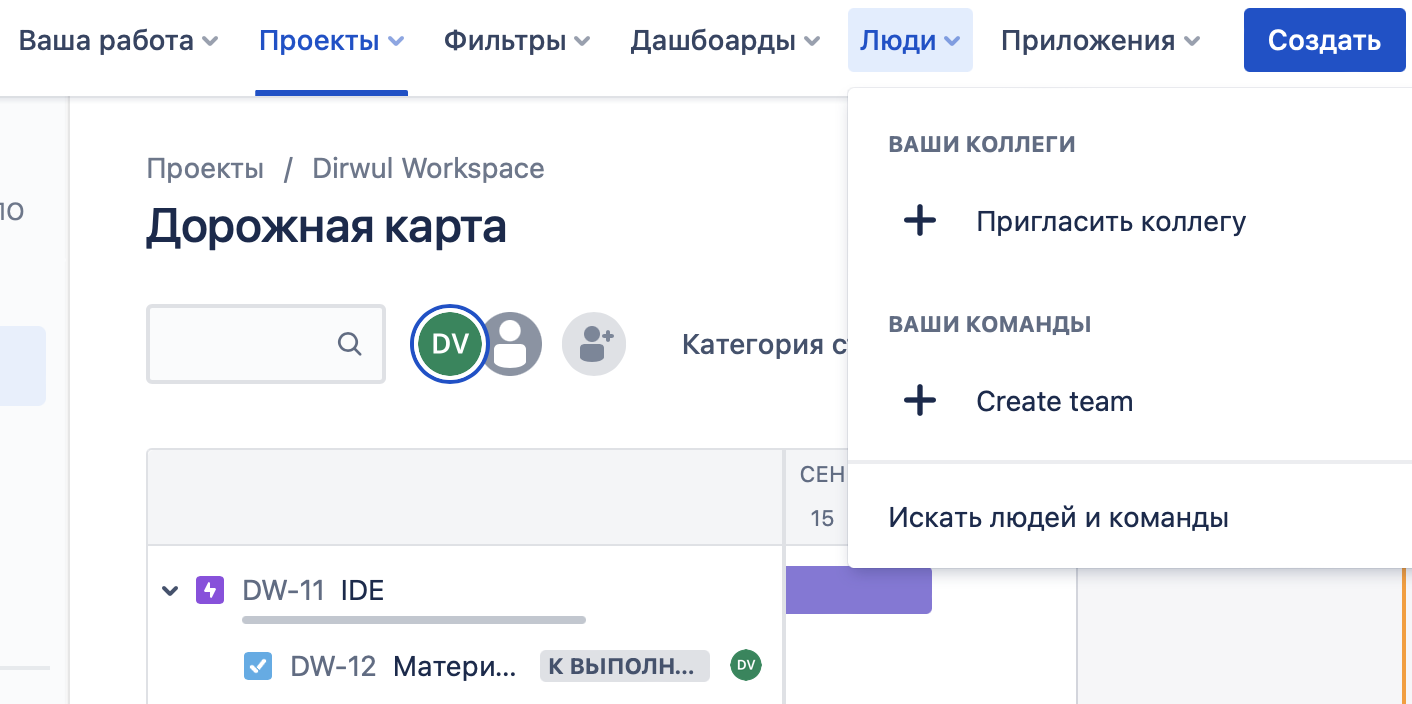
\includegraphics[width=\linewidth]{src/top3.png}}
            \caption{Люди}
        \end{figure}
        \columnbreak
        \begin{figure}[H]
            \centering{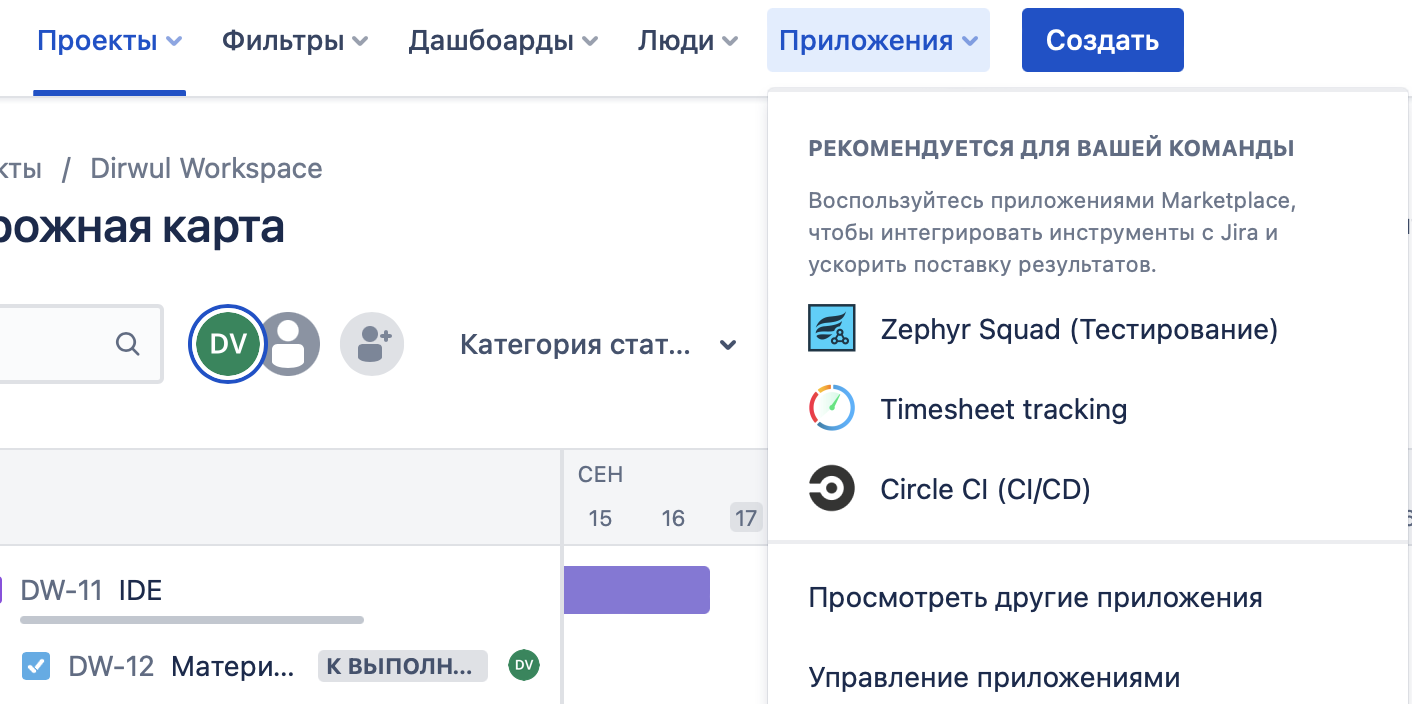
\includegraphics[width=\linewidth]{src/top4.png}}
            \caption{Приложения}
        \end{figure}
    \end{multicols}

\end{document}